% ============================================================
% two-ancilla-checks.tex
% Two-ancilla checks of the folded [[5,1,2]]_3 code, drawn on the paper's
% stabilizer diagrams (fig - 5-qutrit code.tex, panel d, redefined row) with
% the four conventional ancilla sites N, W, E, S filled in.
% (a) the circuits of the earlier two-ancilla runs (code_definitions.py,
%     FoldedQutritSplitAncillaUniformDetectionCode);
% (b) each half on its own ancilla, readouts added afterwards;
% (c) the same split with the two ancillas entangled before coupling;
% (d) the relay through a shared data qutrit that the new two-ancilla runs
%     simulate (FoldedQutritConventionalSitesDetectionCode, worktree
%     conventional-sites): N and E lend, W and S read, every site read once.
% Noiseless checks: naive_split_test.py ((b), (c)), scheduled_sites_test.py and
% data_relay_checks.py ((b) on reused sites, (d)) next to this file.
% ============================================================
\documentclass[tikz,border=4pt]{standalone}
\usepackage{amsmath,amssymb}
\usepackage{pifont}
\usetikzlibrary{calc}

% ---------- palette and sizes (paper: tikz preamble.tex) ----------
\definecolor{Zcol}{HTML}{FF1744}
\definecolor{Xcol}{HTML}{00B7FF}
\definecolor{SwapCol}{HTML}{8E44AD}
\colorlet{Xtint}{Xcol!26}
\colorlet{Ztint}{Zcol!17}
\definecolor{FitCol}{HTML}{009E73}
\colorlet{ClashCol}{Zcol!85!black}
\newcommand{\qdLine}{0.7pt}
\newcommand{\qdR}{4.8pt}
\newcommand{\numFont}{\scriptsize}
\newcommand{\arrAngle}{70}
\newcommand{\arrLen}{0.17cm}
\newcommand{\cmark}{\textcolor{FitCol}{\ding{51}}}
\newcommand{\xmark}{\textcolor{ClashCol}{\ding{55}}}

\newcommand{\WedgeArrow}[2]{%
  \path[fill=black,draw=none]
    ($(#1)+({\qdR*cos(#2+\arrAngle)},{\qdR*sin(#2+\arrAngle)})$)
      arc[start angle=#2+\arrAngle, end angle=#2-\arrAngle, radius=\qdR]
      -- ($(#1)+({(\qdR+\arrLen)*cos(#2)},{(\qdR+\arrLen)*sin(#2)})$) -- cycle;
}

% Patch of the paper's d=2 figure (q2 at the centre) with the conventional
% ancilla sites: N and S on the X-type vertices, W and E on the Z-type faces.
\newcommand{\Patch}{%
  \coordinate (q0) at (-1, 1); \coordinate (q1) at ( 1, 1);
  \coordinate (q2) at ( 0, 0);
  \coordinate (q3) at (-1,-1); \coordinate (q4) at ( 1,-1);
  \coordinate (N) at (0, 1); \coordinate (W) at (-1, 0);
  \coordinate (E) at (1, 0); \coordinate (S) at ( 0,-1);
  \draw[black!22,line width=0.8pt] (q0) -- (q1) (q3) -- (q4) (0,1) -- (0,-1);
}
\newcommand{\Couple}[2]{\draw[line width=1.5pt] (#1) -- (#2);}
\newcommand{\Far}[2]{\draw[ClashCol,line width=1.3pt,dash pattern=on 3pt off 2pt] (#1) -- (#2);}
\newcommand{\Link}[2]{\draw[SwapCol,line width=1.3pt,dash pattern=on 3pt off 2pt] (#1) -- (#2);}
\definecolor{HCol}{HTML}{D35400}
\newcommand{\Lend}[2]{\draw[HCol,line width=1.8pt] (#1) -- (#2);}
% #1 qudits in the check, #2 their fill, #3 the other qudits
\newcommand{\Qudits}[3]{%
  \foreach \i in {#3} {\draw[line width=\qdLine,fill=white] (q\i) circle (\qdR);
                       \node[font=\numFont] at (q\i) {\i};}
  \foreach \i in {#1} {\draw[line width=\qdLine,fill=#2] (q\i) circle (\qdR);
                       \node[font=\numFont,text=white] at (q\i) {\i};}
  \WedgeArrow{q0}{0}\WedgeArrow{q1}{0}\WedgeArrow{q3}{0}\WedgeArrow{q4}{0}\WedgeArrow{q2}{90}
}
\newcommand{\Site}[1]{\node[draw=black!40,dash pattern=on 1.2pt off 1pt,line width=0.5pt,
  fill=white,minimum size=0.28cm,inner sep=0pt] at (#1) {};}
\newcommand{\Anc}[3]{\node[draw=black,line width=0.7pt,fill=#2,minimum size=0.40cm,
  inner sep=0pt,font=\tiny] at (#1) {$#3$};}
\newcommand{\Status}[2]{%
  \node[font=\scriptsize] at (0,-1.50) {#1};
  \node[font=\scriptsize] at (0,-1.88) {#2};
}

\begin{document}
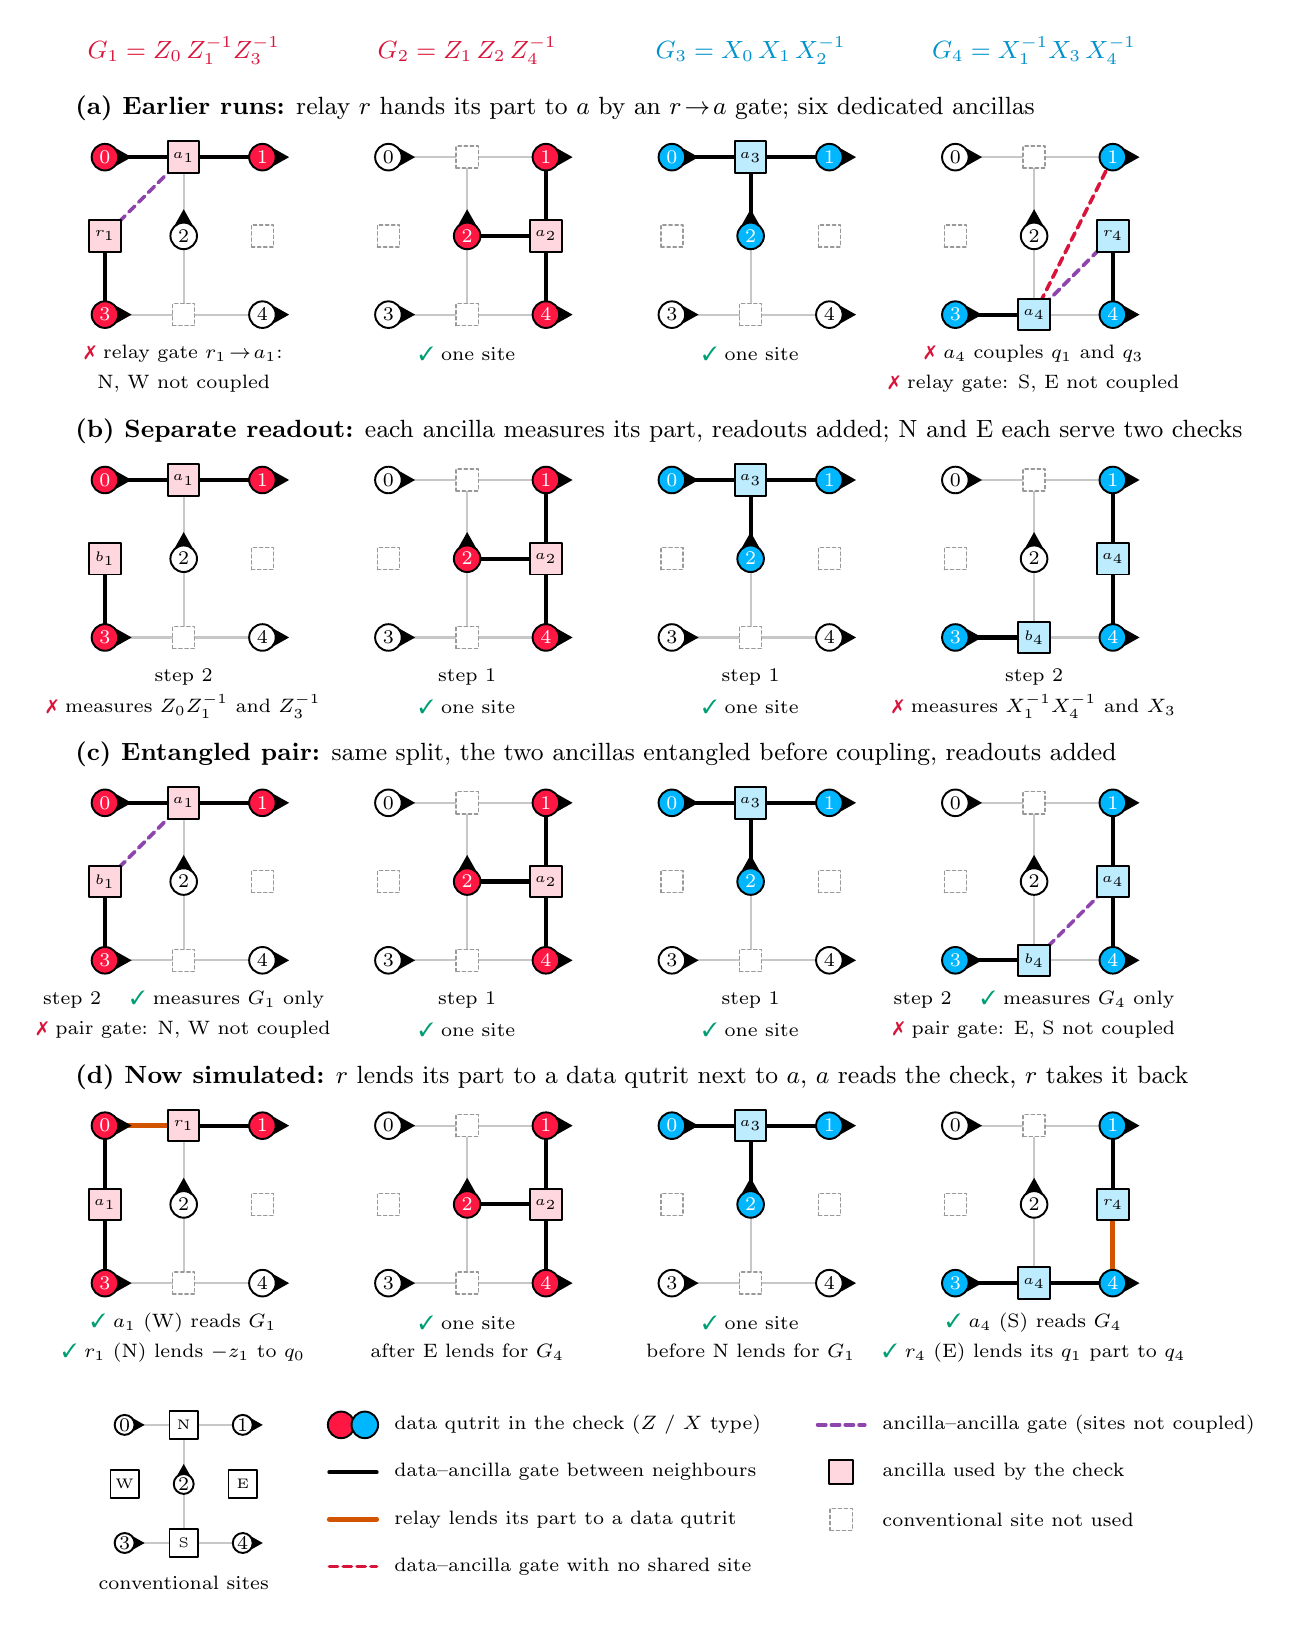
\begin{tikzpicture}[line cap=round,line join=round]
  \def\cA{0} \def\cB{3.6} \def\cC{7.2} \def\cD{10.8}
  \def\rA{0} \def\rB{-4.1} \def\rC{-8.2} \def\rD{-12.3}

  % ---------- column headers ----------
  \node[font=\small,text=Zcol!85!black] at (\cA,2.35) {$G_1 = Z_0\,Z_1^{-1}Z_3^{-1}$};
  \node[font=\small,text=Zcol!85!black] at (\cB,2.35) {$G_2 = Z_1\,Z_2\,Z_4^{-1}$};
  \node[font=\small,text=Xcol!80!black] at (\cC,2.35) {$G_3 = X_0\,X_1\,X_2^{-1}$};
  \node[font=\small,text=Xcol!80!black] at (\cD,2.35) {$G_4 = X_1^{-1}X_3\,X_4^{-1}$};

  % ================= (a) as simulated =================
  \node[anchor=west,font=\small] at (-1.5,\rA+1.62)
    {\textbf{(a) Earlier runs:} relay $r$ hands its part to $a$ by an $r\!\to\!a$ gate; six dedicated ancillas};
  \begin{scope}[shift={(\cA,\rA)}]
    \Patch \Couple{N}{q0} \Couple{N}{q1} \Couple{W}{q3} \Link{N}{W}
    \Qudits{0,1,3}{Zcol}{2,4}
    \Site{E} \Site{S} \Anc{N}{Ztint}{a_1} \Anc{W}{Ztint}{r_1}
    \Status{\xmark\ relay gate $r_1\!\to\!a_1$:}{N, W not coupled}
  \end{scope}
  \begin{scope}[shift={(\cB,\rA)}]
    \Patch \Couple{E}{q1} \Couple{E}{q2} \Couple{E}{q4}
    \Qudits{1,2,4}{Zcol}{0,3}
    \Site{N} \Site{W} \Site{S} \Anc{E}{Ztint}{a_2}
    \Status{\cmark\ one site}{}
  \end{scope}
  \begin{scope}[shift={(\cC,\rA)}]
    \Patch \Couple{N}{q0} \Couple{N}{q1} \Couple{N}{q2}
    \Qudits{0,1,2}{Xcol}{3,4}
    \Site{W} \Site{E} \Site{S} \Anc{N}{Xtint}{a_3}
    \Status{\cmark\ one site}{}
  \end{scope}
  \begin{scope}[shift={(\cD,\rA)}]
    \Patch \Couple{S}{q3} \Far{S}{q1} \Couple{E}{q4} \Link{S}{E}
    \Qudits{1,3,4}{Xcol}{0,2}
    \Site{N} \Site{W} \Anc{S}{Xtint}{a_4} \Anc{E}{Xtint}{r_4}
    \Status{\xmark\ $a_4$ couples $q_1$ and $q_3$}{\xmark\ relay gate: S, E not coupled}
  \end{scope}

  % ================= (b) separate readout =================
  \node[anchor=west,font=\small] at (-1.5,\rB+1.62)
    {\textbf{(b) Separate readout:} each ancilla measures its part, readouts added; N and E each serve two checks};
  \begin{scope}[shift={(\cA,\rB)}]
    \Patch \Couple{N}{q0} \Couple{N}{q1} \Couple{W}{q3}
    \Qudits{0,1,3}{Zcol}{2,4}
    \Site{E} \Site{S} \Anc{N}{Ztint}{a_1} \Anc{W}{Ztint}{b_1}
    \Status{step 2}{\xmark\ measures $Z_0Z_1^{-1}$ and $Z_3^{-1}$}
  \end{scope}
  \begin{scope}[shift={(\cB,\rB)}]
    \Patch \Couple{E}{q1} \Couple{E}{q2} \Couple{E}{q4}
    \Qudits{1,2,4}{Zcol}{0,3}
    \Site{N} \Site{W} \Site{S} \Anc{E}{Ztint}{a_2}
    \Status{step 1}{\cmark\ one site}
  \end{scope}
  \begin{scope}[shift={(\cC,\rB)}]
    \Patch \Couple{N}{q0} \Couple{N}{q1} \Couple{N}{q2}
    \Qudits{0,1,2}{Xcol}{3,4}
    \Site{W} \Site{E} \Site{S} \Anc{N}{Xtint}{a_3}
    \Status{step 1}{\cmark\ one site}
  \end{scope}
  \begin{scope}[shift={(\cD,\rB)}]
    \Patch \Couple{E}{q1} \Couple{E}{q4} \Couple{S}{q3}
    \Qudits{1,3,4}{Xcol}{0,2}
    \Site{N} \Site{W} \Anc{E}{Xtint}{a_4} \Anc{S}{Xtint}{b_4}
    \Status{step 2}{\xmark\ measures $X_1^{-1}X_4^{-1}$ and $X_3$}
  \end{scope}

  % ================= (c) entangled pair =================
  \node[anchor=west,font=\small] at (-1.5,\rC+1.62)
    {\textbf{(c) Entangled pair:} same split, the two ancillas entangled before coupling, readouts added};
  \begin{scope}[shift={(\cA,\rC)}]
    \Patch \Couple{N}{q0} \Couple{N}{q1} \Couple{W}{q3} \Link{N}{W}
    \Qudits{0,1,3}{Zcol}{2,4}
    \Site{E} \Site{S} \Anc{N}{Ztint}{a_1} \Anc{W}{Ztint}{b_1}
    \Status{step 2 \quad \cmark\ measures $G_1$ only}{\xmark\ pair gate: N, W not coupled}
  \end{scope}
  \begin{scope}[shift={(\cB,\rC)}]
    \Patch \Couple{E}{q1} \Couple{E}{q2} \Couple{E}{q4}
    \Qudits{1,2,4}{Zcol}{0,3}
    \Site{N} \Site{W} \Site{S} \Anc{E}{Ztint}{a_2}
    \Status{step 1}{\cmark\ one site}
  \end{scope}
  \begin{scope}[shift={(\cC,\rC)}]
    \Patch \Couple{N}{q0} \Couple{N}{q1} \Couple{N}{q2}
    \Qudits{0,1,2}{Xcol}{3,4}
    \Site{W} \Site{E} \Site{S} \Anc{N}{Xtint}{a_3}
    \Status{step 1}{\cmark\ one site}
  \end{scope}
  \begin{scope}[shift={(\cD,\rC)}]
    \Patch \Couple{E}{q1} \Couple{E}{q4} \Couple{S}{q3} \Link{E}{S}
    \Qudits{1,3,4}{Xcol}{0,2}
    \Site{N} \Site{W} \Anc{E}{Xtint}{a_4} \Anc{S}{Xtint}{b_4}
    \Status{step 2 \quad \cmark\ measures $G_4$ only}{\xmark\ pair gate: E, S not coupled}
  \end{scope}

  % ================= (d) scheduled data relay =================
  \node[anchor=west,font=\small] at (-1.5,\rD+1.62)
    {\textbf{(d) Now simulated:} $r$ lends its part to a data qutrit next to $a$, $a$ reads the check, $r$ takes it back};
  \begin{scope}[shift={(\cA,\rD)}]
    \Patch \Couple{W}{q0} \Couple{W}{q3} \Couple{N}{q1} \Lend{N}{q0}
    \Qudits{0,1,3}{Zcol}{2,4}
    \Site{E} \Site{S} \Anc{W}{Ztint}{a_1} \Anc{N}{Ztint}{r_1}
    \Status{\cmark\ $a_1$ (W) reads $G_1$}{\cmark\ $r_1$ (N) lends $-z_1$ to $q_0$}
  \end{scope}
  \begin{scope}[shift={(\cB,\rD)}]
    \Patch \Couple{E}{q1} \Couple{E}{q2} \Couple{E}{q4}
    \Qudits{1,2,4}{Zcol}{0,3}
    \Site{N} \Site{W} \Site{S} \Anc{E}{Ztint}{a_2}
    \Status{\cmark\ one site}{after E lends for $G_4$}
  \end{scope}
  \begin{scope}[shift={(\cC,\rD)}]
    \Patch \Couple{N}{q0} \Couple{N}{q1} \Couple{N}{q2}
    \Qudits{0,1,2}{Xcol}{3,4}
    \Site{W} \Site{E} \Site{S} \Anc{N}{Xtint}{a_3}
    \Status{\cmark\ one site}{before N lends for $G_1$}
  \end{scope}
  \begin{scope}[shift={(\cD,\rD)}]
    \Patch \Couple{S}{q3} \Couple{S}{q4} \Couple{E}{q1} \Lend{E}{q4}
    \Qudits{1,3,4}{Xcol}{0,2}
    \Site{N} \Site{W} \Anc{S}{Xtint}{a_4} \Anc{E}{Xtint}{r_4}
    \Status{\cmark\ $a_4$ (S) reads $G_4$}{\cmark\ $r_4$ (E) lends its $q_1$ part to $q_4$}
  \end{scope}

  % ================= legend =================
  \begin{scope}[shift={(\cA,-15.85)},scale=0.75]
    \Patch
    \foreach \P/\txt in {q0/0,q1/1,q2/2,q3/3,q4/4} {
      \draw[line width=\qdLine,fill=white] (\P) circle (\qdR);
      \node[font=\numFont] at (\P) {\txt};}
    \WedgeArrow{q0}{0}\WedgeArrow{q1}{0}\WedgeArrow{q3}{0}\WedgeArrow{q4}{0}\WedgeArrow{q2}{90}
    \foreach \P in {N,W,E,S} \node[draw=black,line width=0.6pt,fill=white,minimum size=0.36cm,
      inner sep=0pt,font=\tiny] at (\P) {\P};
  \end{scope}
  \node[font=\scriptsize,align=center] at (\cA,-17.1) {conventional sites};
  \begin{scope}[font=\scriptsize]
    \def\lx{2.0} \def\mx{8.2}
    \draw[line width=\qdLine,fill=Zcol] (\lx,-15.1) circle (\qdR);
    \draw[line width=\qdLine,fill=Xcol] (\lx+0.30,-15.1) circle (\qdR);
    \node[anchor=west] at (\lx+0.55,-15.1) {data qutrit in the check ($Z$ / $X$ type)};
    \draw[line width=1.5pt] (\lx-0.15,-15.7) -- (\lx+0.45,-15.7);
    \node[anchor=west] at (\lx+0.55,-15.7) {data--ancilla gate between neighbours};
    \draw[HCol,line width=1.8pt] (\lx-0.15,-16.3) -- (\lx+0.45,-16.3);
    \node[anchor=west] at (\lx+0.55,-16.3) {relay lends its part to a data qutrit};
    \draw[ClashCol,line width=1.3pt,dash pattern=on 3pt off 2pt] (\lx-0.15,-16.9) -- (\lx+0.45,-16.9);
    \node[anchor=west] at (\lx+0.55,-16.9) {data--ancilla gate with no shared site};
    \draw[SwapCol,line width=1.3pt,dash pattern=on 3pt off 2pt] (\mx-0.15,-15.1) -- (\mx+0.45,-15.1);
    \node[anchor=west] at (\mx+0.55,-15.1) {ancilla--ancilla gate (sites not coupled)};
    \node[draw=black,line width=0.7pt,fill=Ztint,minimum size=0.30cm,inner sep=0pt] at (\mx+0.15,-15.7) {};
    \node[anchor=west] at (\mx+0.55,-15.7) {ancilla used by the check};
    \node[draw=black!40,dash pattern=on 1.2pt off 1pt,line width=0.5pt,minimum size=0.28cm,
      inner sep=0pt] at (\mx+0.15,-16.3) {};
    \node[anchor=west] at (\mx+0.55,-16.3) {conventional site not used};
  \end{scope}
\end{tikzpicture}
\end{document}
